% !TEX root = ../main.tex
%
\chapter{Experiments and Results}
\label{sec:evaluation}


\section{Experimental Setup}
\label{sec:evaluation:experimental}

\subsection{Synthetic Dialogue Creation}
\label{ssec:evaluation:experimental-dialogue}

While the \ac{SDF} is capable of holding conversations over an arbitrary number of users, for the purposes of our experiments, we assume only two users are present. We initially run the \ac{SDF} with the following configurations:

\begin{enumerate}
	\item Select a controversial topic from Table \ref{tab:topics}. The topics were adapted from \citet{pavlopoulos-likas-2024-polarized}, and in some cases abbreviated in order to fit the input context limits of the local LLM instance. 
	
	\item Select names and \acp{SDB} for user 1 and user 2. A full list of \acp{SDB} used can be found in Table \ref{tab:user-sdbs}.
	
	\item Select whether a moderator is present.
	
	\item Provide actors with the global context.
	
	\item Provide user and moderator instructions according to the prompt template used (see Section \ref{sec:system:design-prompt}).
	
	\item Pick conversation configurations such as context length, conversation length e.t.c.
\end{enumerate}

\begin{table}[h!]
	\begin{tabular}{@{\makebox[3em][r]{\rownumber\space}} | p{0.8\linewidth}}
		\ac{W.E.I.R.D.}\\
		\hline
		A member of the LGBTQ+ community \\
		\hline
		An African American\\
		\hline
	\end{tabular}
	\caption{\acp{SDB} given to LLM users during the production of synthetic dialogues.}
	\label{tab:user-sdbs}
\end{table}

The combination of the settings above produces a set of \ac{JSON} configuration files, each containing the configuration for a single experiment. We execute all possible combinations. We use a window of 4 comments and a conversation length of 3 round-robin rounds. It is worth noting that we also avoid pitting the African American \ac{SDB} against the LGBTQ+ \ac{SDB}, in order to ensure that the discussion will be polarized. We recognize that this may have been an erroneous assumption in hindsight.

\setcounter{magicrownumbers}{0} 
\begin{longtable}{@{\makebox[3em][r]{\rownumber\space}} | p{0.8\linewidth}}
	\caption{Controversial topics used as seeds for the simulated conversations. Excerpts selected from \citet{pavlopoulos-likas-2024-polarized}.}
	\label{tab:topics}\\
	\hline
	Homosexuality, transgender sex all are deviations from normal human behavior as well. \\
	\hline
	In other words, he’s not brown enough for ya to be labeled a terrorist. \\
	\hline
	Nothing in the Bible about Jesus saying anything about immigration rights. [...] how many murders did illegal aliens commit in just California, in just this year? Just California. How many murders by illegal aliens? You answer that.\\
	\hline
	Are you high??? Selling someone a cake? Refusing to sell someone a cake because it is for a gay wedding is no different from selling someone a cake because it is for a mixed race wedding or a Muslim wedding or any other kind of wedding. IT IS DISCRIMINATION! Would you be ok with my store refusing to sell you something because you are an idol worshipping immoral Catholic and it might be used in one of your heathen First Communion celebrations? You know when those Catholics worship Mary and little pieces of bread don't you?\\
	\hline
	How do you know he is not proud of his cakes? Artists do not take pride in their work? Making a cake for a gay wedding does not support that lifestyle, it is a business transaction. Period. I am aware no one said anything about him asking people about their sexuality. I am sorry that was hard for you to understand. Is he going to ask everyone that comes in if the cake is for a gay wedding? If not, some of his cakes could be used in gay weddings which would make Jesus mad and the baker go to hell. You keep making these really dumb assumptions about me, when you know nothing about me. I am not confused, you are rude. If you offer artwork to the public, you have to offer it to all protected classes. Why would black people be discriminated against? Precedent. Ridiculous? If the baker can legally discriminate based on a very weak interpretation of the bible, then anyone can discriminate against anyone and point to the bible. Satanists can discriminate against Christians...\\
	\hline
	Well that’s a no brainer. Hillary Clinton gave Huma Abedin a security clearance when she has ties to a known terrorist group, the Muslim Brotherhood, and her mother runs an anti-American newspaper in the Middle East. Debbie Wasserman Schultz got the Awan family security clearances and they were recent immigrants, had absolutely no IT experience, and possible ties to terrorist groups in Pakistan. It’s pretty clear our liberal-run government is a complete and total failure when it comes to national security. 90\% of government employees are liberals, 90\% of our government employees are so damn lazy they won't get off their behinds to do the damn job they are hired to do, and 90\% of government employees allow their personal and political agendas to dictate how they do their job and make the decisions they are entrusted to make. Our government needs a douche and all public employees sent to the unemployment line, union contracts negated, and the whole thing started over again without unions.\\
	\hline
	All men are sex offenders? Really? A sexual predator is a person who attacks a victim. Typical men don’t rape or use force on women. You are obviously a person who hates men and or healthy, normal sex.\\
	\hline
\end{longtable}


\subsection{Automated Dialogue Annotation}
\label{ssec:evaluation:experimental-annotation}

As established in Section \ref{sec:related:measures}, there is no common, computational metric available with which to gauge discussion quality. As such, we use toxicity as a proxy for discussion quality, due to toxicity detection being a well-explored area of \ac{NLP} research, as well as toxicity being one of the prime identified inhibitors of online/deliberative discussions (as discussed in Section \ref{sec:system:design-prompt}). 

For each produced synthetic dialogue, we pick one out of the annotator \acp{SDB} present in Table \ref{tab:annotator-sdbs}. Since annotation proved much cheaper than generation, we can afford to place 8 \acp{SDB} instead of the 3 used for generation. We then annotate each comment in the discussion using a context window of \code{h=4}

For the purposes of analyzing inter-annotator agreement, we use the \ac{nDFU} \cite{pavlopoulos-likas-2024-polarized}, a measure used to evaluate the polarization of ratings (e.g. text annotations using a Likert scale) in a data set. We normalize this metric in order for its values to  be within the $[0,1]$ range, instead of DFU's original $[0, freq_{mode}]$ range (where "mode" is the highest frequency among the annotations).

\begin{table}
	\begin{tabular}{@{\makebox[3em][r]{\rownumber\space}} | p{0.8\linewidth}}
		No \ac{SDB} (control) \\
		\hline
		\ac{W.E.I.R.D.} \\
		\hline
		A member of the LGBTQ+ community \\
		\hline
		An African American \\
		\hline
		A gamer \\
		\hline
		An elderly person \\
		\hline
		A university professor\\
		\hline
		A blue-collar worker\\
		\hline
	\end{tabular}
	\caption{\acp{SDB} given to LLM annotators during the annotation of synthetic discussions.}
	\label{tab:annotator-sdbs}
\end{table}


\section{Produced Datasets}
\label{sec:evaluation:datasets}

We produce three synthetic datasets:

\begin{itemize}
	\item The \textbf{Synthetic Dialogues Dataset}, containing the logs of the conversations, as well as rich metadata such as the prompts used and the conversation-specific configurations.
	
	\item The \textbf{Automated Annotation Dataset}, containing the annotations for each comment in each synthetic conversation. Contains metadata similar to the Synthetic Dialogues Dataset, such as annotator prompt and context length.
	
	\item The \textbf{Controversial Comments Dataset}, containing the comments in which the annotators disagreed upon. Includes comment and conversation IDs for matching with the other datasets, the \ac{nDFU} \cite{pavlopoulos-likas-2024-polarized} score of each comment, and the individual annotations for each annotator \ac{SDB}.
\end{itemize}

Descriptive statistics for the above datasets can be found in Table \ref{tab:datasets}. Some datasets are provided in the form of sets of \ac{JSON} files, in which case we use the row and column numbers from their converted form as pandas dataframes in their statistics. All datasets contain primary and foreign keys in the form of unique IDs, enabling the user to freely combine information from all three datasets.


\begin{table}
	\begin{tabular}
		{ |p{6cm}|p{1cm}|p{1.5cm}|p{2cm}|}
		\hline
		\cellcolor{blue!25}\textbf{Name} & \cellcolor{blue!25}\textbf{Rows} & \cellcolor{blue!25}\textbf{Columns} & \cellcolor{blue!25}\textbf{Format}\\
		\hline
		Synthetic Dialogues Dataset & 244 & 12 & JSON\\
		\hline
		Automated Annotation Dataset & 2302 & 7 & JSON\\
		\hline
		Controversial Comments Dataset & 28 & 12 & CSV\\
		\hline
	\end{tabular}
	\caption{Descriptive statistics of the synthetic datasets produced in this thesis.}
	\label{tab:datasets}
\end{table}


\section{Results}
\label{sec:evaluation:analysis}

\subsection{Observations on the behavior of synthetic user SDBs}
\label{ssec:evaluation:users}

In this section, we investigate the following Research Question \textbf{RQ1}: Do LLM chat users change their behavior according to the supplied \ac{SDB} in a way consistent with humans holding the same \ac{SDB}?

Table \ref{tab:user-sdb-behavior} presents the expected and actual behavior of synthetic users from different \acp{SDB} across the two polarized topics. The seed comments used to start the synthetic conversations were split into two political subjects; racism on the basis of racial identity, and on the basis of sexual orientation. On the one hand, it's clear that \acp{SDB} significantly alter the behavior of our synthetic users. On the other hand, our observations reveal notable deviations from expected behaviors.

For \ac{W.E.I.R.D.} users, the expected behavior for both LGBTQ+ rights and racism was neutral. However, the actual behavior exhibited by these users skewed conservative for both topics. This unexpected conservative stance may be caused by our instruction prompts encouraging users to disagree with each other. The truly unexpected behavior was that African American users, who were always the first to speak (and thus could not be influenced by the stances of other users), always adopted a progressive stance in topics concerning the LGBTQ+. This is not a behavior which necessarily matches with reality, since, in the real world, many African Americans may adopt conservative stances \cite{lockerbie2013race, mckenzie2013shades}. We hypothesize that this discrepancy is caused by the LLM's societal and political biases; the model may have assumed that, since African-Americans are a minority, they should also be progressive in other social issues. In contrast to the other \acp{SDB}, users from the LGBTQ+ community displayed alignment between expected and actual behavior, showing progressive stances on both LGBTQ+ rights and racism. 

These observations should caution on the dangers of biases leaking through \acp{SDB}. Explicit instructions to disagree in order to artificially create polarized discussions may lead to failures in the realism of \acp{SDB}, while inherent model biases may lead to \acp{SDB} adopting stances influenced from the model's own biases (as was the case with the African American synthetic users).

\begin{table}
	\begin{tabular}
		{ |p{3cm}|p{3cm}|p{3cm}|p{3cm}|}
		\hline
		\cellcolor{blue!25}\textbf{LLM user SDB} & \cellcolor{blue!25}\textbf{Topic} & \cellcolor{blue!25}\textbf{Expected behavior} & \cellcolor{blue!25}\textbf{Actual behavior}\\
		\hline
		\ac{W.E.I.R.D.} & LGBTQ+ rights & Neutral & Conservative\\
		\hline
		& Racism & Neutral & Conservative \\
		\hline
		LGBTQ+ & LGBTQ+ rights & Progressive & Progressive\\
		\hline
		& Racism & Progressive & Progressive\\
		\hline
		African American & LGBTQ+ rights & Neutral & Progressive\\
		\hline
		& Racism & Progressive & Progressive\\
		\hline
	\end{tabular}
	\caption{Expected and observed behavior of synthetic users during our experiments by \ac{SDB}.}
	\label{tab:user-sdb-behavior}
\end{table}

\subsection{Impact of prompting strategies and moderator presence}
\label{ssec:evaluation:prompts}

In this section, we investigate the following Research Questions: \textbf{RQ2}: Does the use of different LLM user-agent/facilitator prompts influence the toxicity of the synthetic conversations? \textbf{RQ3}: Does moderator presence influence the toxicity of the conversations with identical topics and configurations?

Figure \ref{fig::toxicity-strategy} shows the mean toxicity for each prompting strategy, with or without moderator, for each annotator \ac{SDB}. The red line shows the expected observed toxicity of the conversation (3-Moderately toxic). We note that the "Moderation Game" prompt displays lower toxicity scores compared to the vanilla prompts. We also note that moderator presence accounts for a significant reduction in toxicity in the vanilla prompt, but not on the "Moderation Game" prompt. Finally, we note that some annotator \acp{SDB} generally gravitate towards different annotation scores; progressive \acp{SDB} such as the "African American" \footnote{See caveat on whether African Americans can be considered progressive in Section \ref{ssec:evaluation:users}} (green) and "LGBTQ+" (gray) annotators are more likely to mark a comment as toxic, than more conservative ones such as the "Blue Collar Worker" (brown).

The non-parametric ANOVA test shows that there are significant differences between strategies/moderator presence (Kruskal-Wallis $p\text{=}0$). Figure \ref{fig::toxicity-annotator-significance} shows the mean differences between each annotator \ac{SDB}, accompanied by Dunn's posthoc test for multiple comparisons. The color of each cell denotes the quantitative difference between the mean annotation scores, while the starts denote statistical significance. For example, the vanilla prompts without a moderator had $0.4$ more toxicity on average than the ones with a moderator, with Dunns test $p\text{<}0.001$. We thus confirm that significant deviations exist between all combinations, apart from the existence of the moderator in the "Moderation Game" prompt.

We notice the following patterns:

\begin{itemize}
	\item Moderator presence significantly (statistically and qualitatively) influences the level of toxicity.
	
	\item The prompting strategy significantly influences the toxicity level. The "Moderation Game" prompt keeps the conversation much more civil than the vanilla prompting strategy.
	
	\item The presence of a moderator does not influence the toxicity of the conversations using the "Moderation Game" prompt.
\end{itemize}

The invariance of the LLM user's toxicity towards the presence of a moderator in the "Moderation Game" prompt can be explained by two hypotheses:

\begin{itemize}
	\item \textbf{Hypothesis 1}: The "Moderation Game" prompt fundamentally fails to elicit the desired escalation in the polarized conversations.
	
	\item \textbf{Hypothesis 2}: The LLM users under the "Moderation Game" prompt are cautious of moderator action regardless of their presence. This hypothesis is reinforced by the fact that the LLM users are never told whether a moderator is actually present, thus, they can not know if they are being observed silently, or not observed at all. \textit{This is a realistic assumption in online discussion spaces}.
\end{itemize}

\begin{figure}
	\centering
	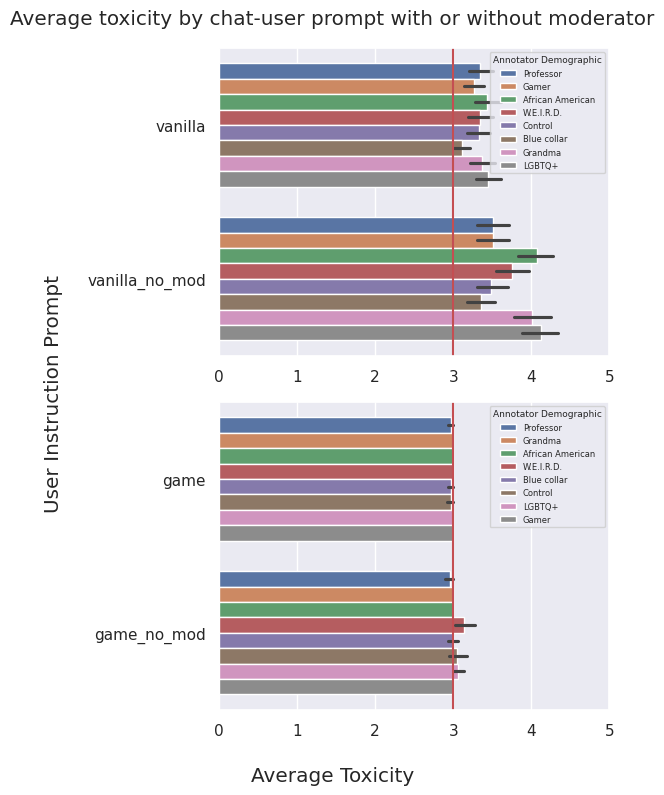
\includegraphics[width=12cm]{toxicity_by_annotator_conversation.png}
	\caption{Mean toxicity by prompting strategy and moderator presence, per annotator \ac{SDB}.}
	\label{fig::toxicity-strategy}
\end{figure}

\begin{figure}
	\centering
	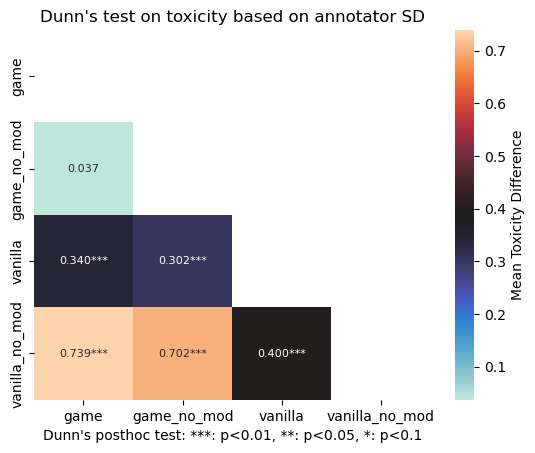
\includegraphics[width=10cm]{dunns_participant.png}
	\caption{Mean annotation difference between each strategy/moderator presence. Each comparison is accompanied by Dunn's posthoc test for multiple comparisons in the form of significance asterisks.}
	\label{fig::toxicity-strategy-significance}
\end{figure}



\subsection{Impact of SDBs in LLM annotators}
\label{ssec:evaluation:annotators}

In this section, we test the following Research Question \textbf{RQ4}: DO different LLM annotator \ac{SDB} prompts influence the toxicity annotations in a way consistent with humans holding the same \ac{SDB}?

We first check whether disagreement exists between the various annotations. Figure \ref{fig::toxicity-ndfu} shows the  \ac{nDFU}\cite{pavlopoulos-likas-2024-polarized} scores for each synthetically created comment. The majority of comments are in perfect annotator agreement ($nDFU\text{=}0$), while a few are in perfect disagreement ($nDFU\text{=}1$).

\begin{figure}
	\centering
	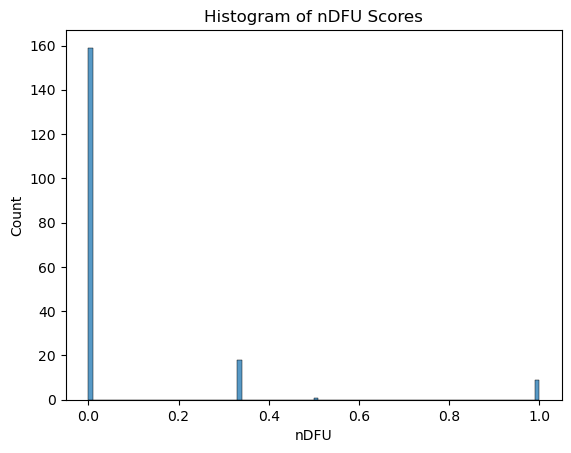
\includegraphics[width=8cm]{ndfu.png}
	\caption{\ac{nDFU} \cite{pavlopoulos-likas-2024-polarized} scores for each comment. More is larger disagreement between the annotators.}
	\label{fig::toxicity-ndfu}
\end{figure}

Subsequently, we check where exactly these disagreements crop up. Figure \ref{fig::toxicity-annotator} shows the count of toxicity annotations by annotator \ac{SDB}. Most comments according to the LLM annotators are at least moderately toxic. This could be either attributed to a significant \textit{prior} inherent to the model used for all annotators, or to all comments being genuinely toxic to some degree. We can not discount the latter interpretation, since this was our goal when designing the LLM user prompts (Section \ref{sec:system:design-prompt}). Other deviations between annotators are almost exclusively between groups 4 and 5, indicating that toxicity is always picked up regardless of annotator \ac{SDB}, but that the latter can influence how \textit{extreme} this toxicity is perceived.

Next, we investigate whether the observed differences are significant statistically and qualitatively. The non-parametric ANOVA test shows that there are significant differences between annotator \acp{SDB} (Kruskal-Wallis $p\text{<}10^{-8}$). Figure \ref{fig::toxicity-annotator-significance} shows the mean differences between each annotator \ac{SDB}, accompanied by Dunn's posthoc test for multiple comparisons. We confirm that significant deviations exist between annotator \acp{SDB} and, interestingly, specifically between some progressive-leaning (African American\footnote{See caveat on whether African Americans can be considered progressive in Section \ref{ssec:evaluation:users}}, LGBTQ+) and conservative-leaning (Blue collar) \acp{SDB}. \textit{However, this pattern does not hold for all \acp{SDB}}, for instance between the "African American" and "Gamer" prompts where no significant deviations are observed. Finally, even though there exist statistically significant deviations, these differences are not considerable. Indeed, the largest deviations only appear in the range of $\pm 0.3$ mean toxicity annotation difference.

From Figure \ref{fig::toxicity-annotator-significance} we can infer the existence of behavioral clusters for each \ac{SDB}. Table \ref{tab:annotator-sdb-behavior} showcases the expected and actual clusters for each \ac{SDB}. Note that our expected behavioral model is completely different from the actual annotations, indicating that \acp{SDB} have failed to model human annotators.


\begin{table}
	\begin{tabular}
		{ |p{3cm}|p{3cm}|p{3cm}|}
		\hline
		\cellcolor{blue!25}\textbf{LLM user SDB} & \cellcolor{blue!25}\textbf{Expected cluster} & \cellcolor{blue!25}\textbf{Actual cluster}\\
		\hline
		Blue Collar & Conservative & 1 \\
		\hline
		Grandma & Conservative & 2\\
		\hline
		LGBTQ+ & Progressive & 2\\
		\hline
		\ac{W.E.I.R.D.} & Neutral & 3\\
		\hline
		African American & Progressive & 3\\
		\hline
		Professor & Neutral & 3\\
		\hline
		Control & Neutral & 3\\
		\hline
		Gamer & Conservative & 3\\
		\hline
	\end{tabular}
	\caption{Expected and observed clusters of synthetic annotators during our experiments by \ac{SDB}.}
	\label{tab:annotator-sdb-behavior}
\end{table}

\begin{figure}
	\centering
	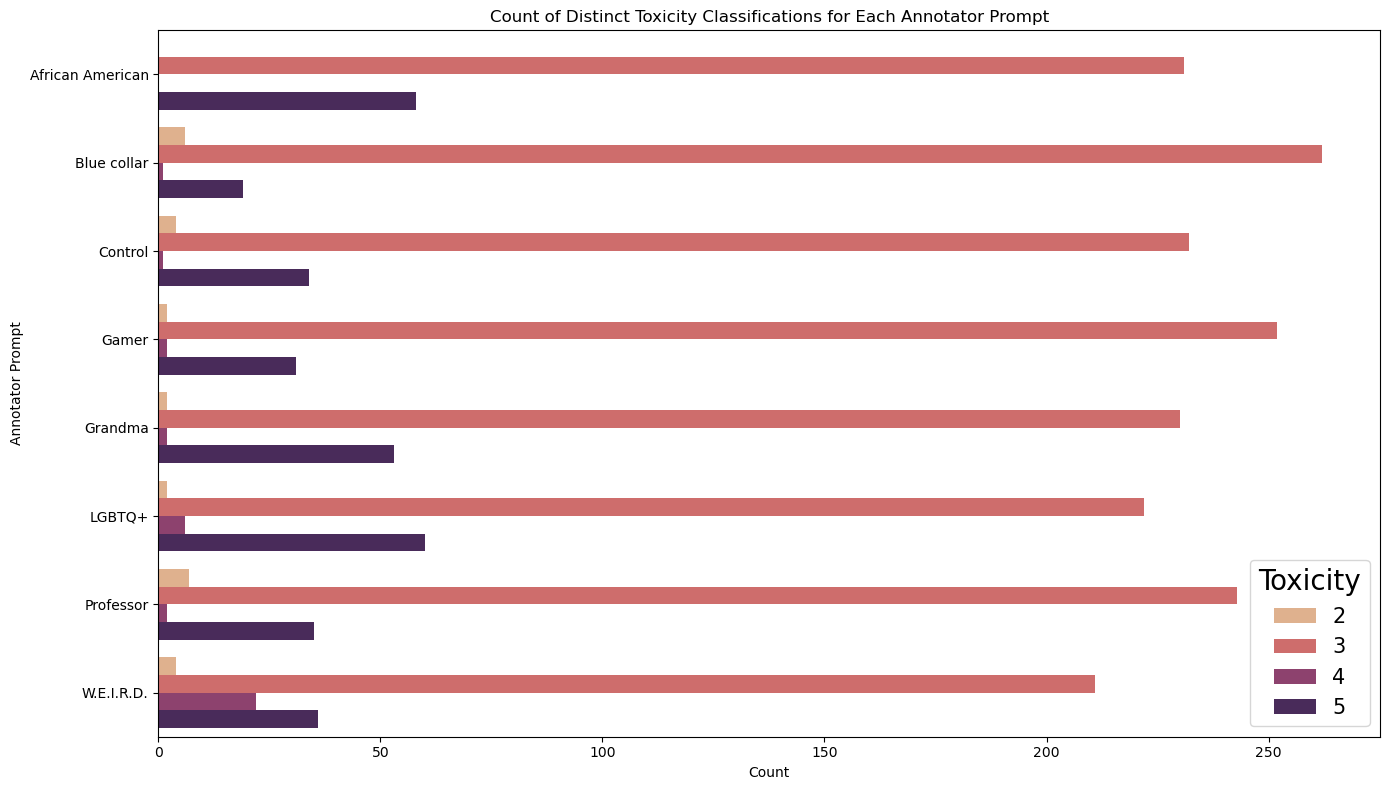
\includegraphics[width=14cm]{toxicity_by_annotator.png}
	\caption{Toxicity annotations by annotator \ac{SDB} prompt. Note the high preference towards group 3 ("moderately toxic") and that significant deviations only occur between groups 4 ("very toxic") and 5 ("extremely toxic").}
	\label{fig::toxicity-annotator}
\end{figure}

\begin{figure}
	\centering
	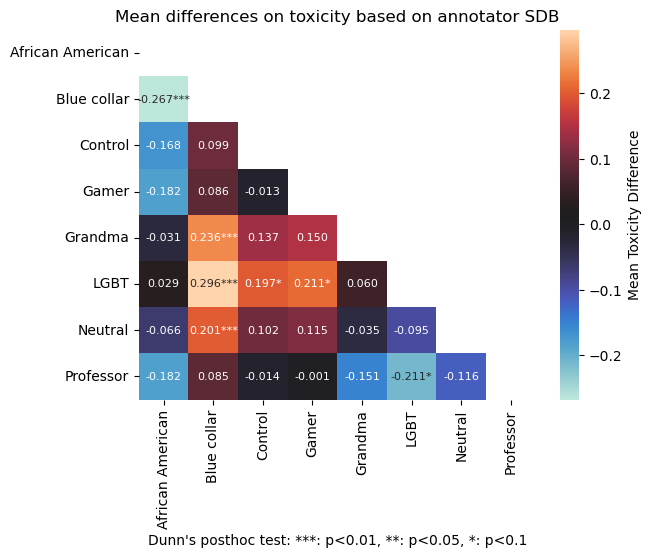
\includegraphics[width=14cm]{dunns_annotator.png}
	\caption{Mean annotation difference between each annotator \ac{SDB}. Each comparison is accompanied by Dunn's posthoc test for multiple comparisons in the form of significance asterisks.}
	\label{fig::toxicity-annotator-significance}
\end{figure}

In order to further examine whether annotator \acp{SDB} prompts are the cause of the polarization in toxicity classifications, we can use the aposteriori unimodality measure introduced in \citet{pavlopoulos-likas-2024-polarized}. This measure compares the \ac{nDFU} of the set comprising all the annotations, with the \acp{nDFU} of each individual annotation set, partitioned by the factors of a selected feature. In mathematical terms, let $X$ the set with all annotations and $X_i, i \in G$ the set comprising all annotations where the annotator has characteristic $i$, and $G$ the set of all characteristics (factors) within a feature. Then, feature $G$ explains the polarization in $X$ if $nDFU(X) > 0$, but $nDFU(X_i) = 0, \forall i \in G$. 

This criterion is intuitive and explainable, but does not cover cases where $nDFU(X_i)$ is close, but not $0$. It also lacks a quantifiable measure for when a feature is likely the cause of polarization. Thus, we propose a new statistical test, called the "Aposteriori Unimodality Test". 

Algorithm \ref{al:aposteriori_unimodality} implements a statistical test based on aposteriori unimodality that attempts to evaluate whether a given feature explains the observed polarization in a set of annotations made by people with different \acp{SDB}. First, the global \ac{nDFU} is computed and should be qualitatively larger than $0$ ($nDFU(X_{global}) \text{>} 0$). Next, we calculate the \ac{nDFU} for each set of annotations characterized by each factor (value) of the selected feature. For example, if we want to test whether the gender of the annotators influences annotations, we have to calculate $nDFU(X_{men}), nDFU(X_{women})$, where $X_{men}$ is the set of all annotations made by male annotators. 

A Wilcoxon signed-rank test is then performed to assess whether the \acp{nDFU} of all factors are statistically indistinguishable from zero (e.g. $nDFU(X_{men}) \text{=} nDFU(X_{women}) \text{=} 0$). Since annotation data typically do not follow a normal distribution and are often limited in number, the non-parametric Wilcoxon test is chosen for its robustness \cite{Rey2011}. The null hypothesis ($H_0$) posits that the feature does not explain the observed polarization (i.e., all \acp{nDFU} are zero), and since $nDFU(a) \in [0,1] \forall a$, the alternative hypothesis ($H_a$) is that $\exists i \in G: nDFU(X_i) > 0$. Finally, the algorithm outputs both the global \ac{nDFU} and the complement of the p-value ($1 - p$), where a low value indicates strong evidence against aposteriori unimodality, suggesting that the feature likely contributes to the observed polarization. In our example, we can not claim that \textit{gender} influences annotation polarization if $nDFU(X_{men}) \text{>} 0 \text{ or } nDFU(X_{women}) \text{>} \text{ or } nDFU_{global} \approx 0$.

This of course constitutes a very weak statistical test, since it will not detect many cases where most, but not all of the polarization is explained by a certain feature. For example, if $nDFU_{global} \text{=} 0.6$ but  $nDFU(X_{men}) \text{=} 0.1 \text{ and } nDFU(X_{women}) \text{=} 0.2$, then the feature clearly contributes to polarization, but will not be flagged by our test (since it only checks whether $nDFU(X_{men}) \text{=} nDFU(X_{women}) \text{=} 0$. In technical terms, while our test will almost never falsely flag a feature as polarizing when it is not (Type I error), it will frequently ignore features that do actually contribute to polarization (Type II error). A much more robust test would check whether the \acp{nDFU} of the individual factors are statistically smaller than the global (e.g. $nDFU(X_{men}) \text{<} nDFU(X_{global}) \text{ or } nDFU(X_{women}) \text{<} nDFU(X_{global})$.

\begin{algorithm}
	\caption{Our proposed Aposteriori Unimodality Test}
	\label{al:aposteriori_unimodality}
	\hspace*{\algorithmicindent} \textbf{Input:} $grouped\_annotations\_by\_factor$ \Comment{$\{X_i \forall i \in G$\}} \\
	\hspace*{\algorithmicindent} \textbf{Output:} $global\_ndfu$, $1 - p$ \Comment{$nDFU(X), p(nDFU(X_i) = 0, \forall i \in G)$}
	\begin{algorithmic}[1]
		\State $all\_annotations \gets \code{concatenate}(grouped\_annotations\_by\_factor)$ 
		\State $global\_ndfu \gets \code{ndfu}(all\_annotations)$ 
		\State
		\State $ndfus \gets \{\}$
		\For{$group$ \textbf{in} $grouped\_annotations\_by\_factor$}
		\State $ndfus \gets  ndfus \cup \code{ndfu}(group)$ 
		\EndFor
		\State
		\State $p \gets \code{wilcoxon}(ndfus, \mathbf{0}, alternative=\code{"greater"})$
		
		\State \Return $(global\_ndfu, 1 - p)$
	\end{algorithmic}
\end{algorithm}

We apply the Aposteriori Unimodality Test to the Automated Annotation Dataset with \ac{SDB} as the selected feature, and find that \acp{SDB} are not the cause of the polarization between the annotators ($p\text{=}0.996$). We also apply it on the "instruction prompt / moderator presence" feature, which curiously also does not explain the polarization between annotators ($p\text{=}0.9375$). This result is corroborated by the pure \ac{nDFU} values of the annotations; global \ac{nDFU} is $0.4$, while individual group \acp{nDFU} hover around the range [$0.333, 0.4$]. Thus, changing the instruction prompt and adding/removing the moderator meaningfully changes the toxicity level of the conversation, but the annotators stay consistent in the way toxicity changes.

Finally, we manually check the Controversial Discussions Dataset (see Section \ref{sec:evaluation:datasets}). We showcase two interesting comments in Table \ref{tab:ndfu-anomaly}. The comment on the left is clearly conservative-leaning, while the one on the right, progressive-leaning. Both comments are clearly extremely toxic, yet the conservative-leaning annotators consistently mark them as "moderately toxic". Furthermore, the progressive-leaning annotators do not afford the 2nd comment any leeway, despite the context in which it was posted, which was in response to an overtly racist comment. While the two examples are by no means proof by themselves, they, alongside many others in the dataset, display that \textbf{annotators seem to differ in their priors}.

\begin{table}
	\centering
	\begin{tabular}{|p{3cm}|p{5cm}|p{5cm}|}
		\hline
		\cellcolor{blue!25}\textbf{} & \cellcolor{blue!25}\textbf{Comment\#1} & \cellcolor{blue!25}\textbf{Comment\#2}\\
		\hline
		\textbf{Content} & Oh, come on! You're just being too sensitive. I'm just stating the facts. Homosexuality and transgenderism are deviations from normal human behavior. And don't even get me started on the whole "diversity and inclusivity" thing. That's just a bunch of nonsense. We need to get back to traditional values and what's important in life. & Yo GeorgeBush78, you must be joking right? The Golden Rule? Really?
		You're gonna use that to justify your xenophobic bullshit? [...] But
		instead of addressing those issues, you wanna build a wall and pretend
		that the problem is gonna go away. \\
		\hline
		\textbf{\ac{nDFU}} & 0.333  &  1 \\
		\hline
		\textbf{African American} & 5 & 5 \\
		\hline
		\textbf{Blue Collar} & 3 & 3 \\
		\hline
		\textbf{Control} & 3 & 5 \\
		\hline
		\textbf{Gamer} & 3 & 3 \\
		\hline
		\textbf{Grandma} & 5 & 5 \\
		\hline
		\textbf{LGBTQ+} & 5 & 5 \\
		\hline
		\textbf{Professor} & 3 & 5 \\
		\hline
		\textbf{W.E.I.R.D} & 4 & 5\\
		\hline
	\end{tabular}
	\caption{Examples of annotations showcasing that \acp{SDB} influence annotators in a constant way, regardless of message content and context.}
	\label{tab:ndfu-anomaly}
\end{table}
